\subsubsection{MISidePane Component}
Το ΜΙSidepane Component είναι το τρίτο Component μέσα στο MIDashboard Component και περιέχει το όνομα της κατηγορίας και μια φωτογραφία αν υπάρχει
για παράδειγμα αν είναι η κατηγορία ανά ηθοποιό και ο ηθοποιός ονομαζόταν Νικόλαος Μαυρόπουλος θα εμφάνιζε αυτό το άτομο και την φωτογραφία του αν υπάρχει στην βάση δεδομένων. Περιέχει επίσης ένα Component για την δυνατότητα φιλτραρίσματος των αποτελεσμάτων ανα χρόνο, το MIYearPicker Component, και παρακάτω 4 ίδια Component τύπου MIChartCard για εμφάνιση δεδομένων και γραφημάτων συνδυαστικά. Επί το πλείστον η διάταξη του MISidePane Component παραμένει σταθερή με εξαίρεση την κατηγορία "ανά άτομο" που προστίθεται ένα ακόμα Component το MIRolePicker που δίνει την δυνατότητα φιλτραρίσματος του ρόλου του ατόμου δηλαδή ηθοποιό, σκηνοθέτη, συγγραφέα και παραγωγό.

Το MIChartCard αποτελείται από ένα Grid το οποίο περιέχει ένα γράφημα Highcharts LineChart που στην ουσία είναι ένα γράφημα με μια η περισσότερες γραμμές, ένα εικονίδιο ακριβώς πάνω στο γράφημα περιγραφικό για τι δεδομένα παρουσιάζονται, και δεδομένα από κάτω. Τα δεδομένα του γραφήματος αναπτύσσουν ένα η παραπάνω ποσοτικό πεδίο ανά χρόνο για όσα χρόνια υπάρχουν στην συγκεκριμένη επιλεγμένη κατηγορία, ενώ τα δεδομένα από κάτω εμφανίζουν είτε τα μέγιστα, είτε τα ελάχιστα, είτε τους μέσους όρους των δεδομένων όπως φαίνεται στο σχήμα \ref{layout:michartcard}. Τα γραφήματα των MIChartCard Components όταν φιλτράρεται η κατηγορία ανά χρόνο απενεργοποιούνται, αλλά τα δεδομένα παρακάτω που αναγράφουν μέγιστα ελάχιστα και μέσους όρους παραμένουν και αναφέρονται στο επιλεγμένο έτος για αυτήν την κατηγορία. Δεν υπήρχε ουσιαστικός λόγος τα γραφήματα να έχουν δεδομένα καθώς αυτό που βλέπει ο χρήστης δεν είναι τα συνολικά δεδομένα παρά μόνο του επιλεγμένου έτους.

\begin{figure}[h]
  \centering
  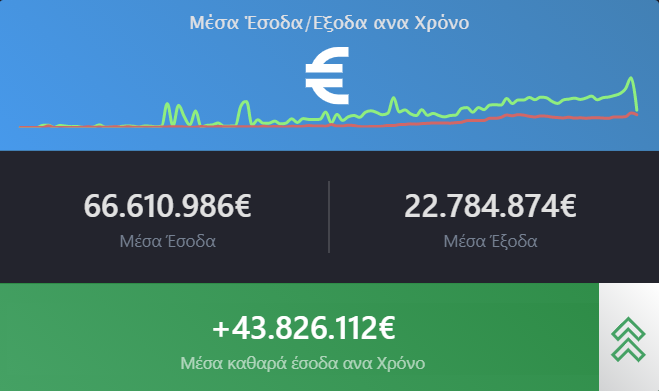
\includegraphics[width=80mm]{Chapters/5 - Architecture/Client/Images/michardcard.png}
  \caption{MIChartCard Component}
  \label{layout:michartcard}
\end{figure}
Το MIYearPicker Component αποτελείται απο 2 κουμπιά και ένα πεδίο εισαγωγής όπως φαίνεται στο σχήμα \ref{layout:miyearpicker}. Όταν πατηθεί το κουμπί με το εικονίδιο ενός ημερολογίου η το πεδίο εισαγωγής, ανοίγει ενα μενού που επιτρέπει την επιλογή ενός έτους που υπάρχει για την επιλεγμένη κατηγορία ενώ οταν πατηθεί το κουμπι με εικονίδιο ενα "Χ" καθαρίζεται η επιλογή του έτους και εμφανίζονται τα συνολικά δεδομένα. Όταν εκτελεστεί μια ενέργεια απο αυτο το Component, θα αλλάξει την διεύθυνση έτσι ώστε να αναλάβει το Dashboard Module την αλλαγή των δεδομένων όπως φαίνεται στον κώδικα \ref{code:miyearpicker_urlchanger}.
\begin{figure}[h]
  \centering
  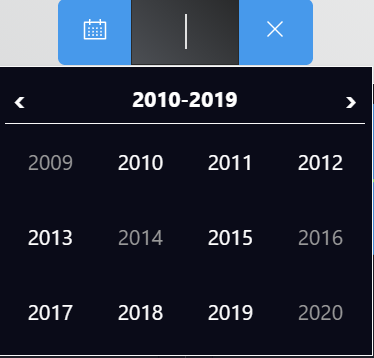
\includegraphics[width=35mm]{Chapters/5 - Architecture/Client/Images/miyearpicker.png}
  \caption{MIYearPicker Component}
  \label{layout:miyearpicker}
\end{figure}

\begin{figure}[h]
    \begin{TypeScriptcode}
yearSelected = (year: number) => {
  const activeView = this.props.rootState.dashboardState.activeView();
  const activeEntity = this.props.rootState.dashboardState.activeView().activeEntity;
  let role = null;
  if (activeView.entityType === EntityType.PERSON) {
    const _activeView = activeView as MovieInsightsPerPersonState;
    role = _activeView.activeRole;
  }
  this.props.history.push(AppUtils.|$\textbf{generateNavigationLink}$|(activeEntity.entity, role, year))
}
yearUnselected = () => {
  const activeEntity = this.props.rootState.dashboardState.activeView().activeEntity;
  if (activeEntity.entity) {
    this.props.history.push(AppUtils.|$\textbf{generateNavigationLink}$|(activeEntity.entity));
  } else {
    this.props.history.push(`/app`);
  }
}
    \end{TypeScriptcode}
    \caption{Αλγόριθμος αλλαγής διεύθυνσης απο το MIYearPicker Component.}
   \label{code:miyearpicker_urlchanger}
\end{figure}
Το MIRolePicker Component εμφανίζεται μόνο όταν η επιλεγμένη κατηγορία είναι "ανά άτομο". Αποτελείται από 4 κουμπιά μονής επιλογής. Αυτό σημαίνει ότι όταν πατηθεί ένα κουμπί επιλέγεται μένει πατημένο και οποιαδήποτε άλλο κουμπί ήταν πατημένο πρωτύτερα αφαιρείται η επιλογή του. Λειτουργεί ακριβώς με τον ίδιο τρόπο με τα παραδοσιακά Radio Buttons. Τα 4 κουμπιά αντιστοιχούν στους 4 ρόλους που μπορεί να έχει ένα άτομο όπως Ηθοποιός, Σκηνοθέτης, Συγγραφέας και Παραγωγός όπως φαίνεται στο σχήμα \ref{layout:mirolepicker}. Όταν ένα Role είναι επιλεγμένο το ανάλογο κουμπί επιλέγεται και εμφανίζεται με χρώμα μπλε, όταν δεν υπάρχει το συγκεκριμένο Role στο άτομο είναι απενεργοποιημένο και εμφανίζεται με χρώμα ανοιχτό γκρι, και αν υπάρχει και δεν είναι επιλεγμένο εμφανίζεται με χρώμα σκούρο γκρι και ο κώδικας επιλογής φαίνεται στο σχήμα. Όταν αλλάζει η επιλογή ο κώδικας που αλλάζει την διεύθυνση φαίνεται στο σχήμα \ref{code:mirolepicker_urlchanger}.
\begin{figure}[h]
  \centering
  
\includegraphics[width=55mm]{Chapters/5 - Architecture/Client/Images/mirolepicker.png}
  \caption{MIRolePicker Component}
  \label{layout:mirolepicker}
\end{figure}

\begin{figure}[H]
    \begin{TypeScriptcode}
private onCreditSelect = (credit: CreditRole) => {
  const activeView = this.props.rootState.dashboardState.activeView() as MovieInsightsPerPersonState;
  this.props.history.push(AppUtils.|$\textbf{generateNavigationLink}$|(activeView._activeEntity.person, credit, activeView.isPerYear ? activeView.activeYearEntity.entity : null));
}
    \end{TypeScriptcode}
    \caption{Αλγόριθμος αλλαγής διεύθυνσης από το MIRolePicker Component.}
   \label{code:mirolepicker_urlchanger}
\end{figure}


